\documentclass[../ECON-281-Notes.tex]{subfiles}
\begin{document}
\chapter{Perfect Competition}
In this chapter we will learn about 
\begin{itemize}
  \item What are the characteristics of perfect competition 
  \item Demand curve of a competitive firm 
  \item Profit maximization 
  \begin{itemize}
    \item Marginal Approach
    \item Total Revenue minus Total Cost approach
  \end{itemize}
  3 cases
  \begin{itemize}
    \item profit
    \item loss - 3 actions
    \begin{itemize}
      \item continue
      \item indifferent
      \item shutdown
    \end{itemize}
    \item breakeven
  \end{itemize}
  \item Short run supply curve of a competitive firm
  \item Long run equilibrium 
  \item Perfect competition and efficiency
\end{itemize}

\section{Characteristic of a perfect competition}
There are 4 characteristics:
\begin{enumerate}
  \item Large number of sellers and buyers.
  \item Sellers sell identical "homogeneous" products.
  \item No single seller controls the price, the market determines the price and the sellers are the \underline{price takers}.
  \item Free entry and exit, i.e., no barrier to entry or exit. In the long run there is no profit nor loss therefore the market of producers in long run  will only have breakeven for profits.
\end{enumerate}

\begin{figure}[!h]
  \centering
  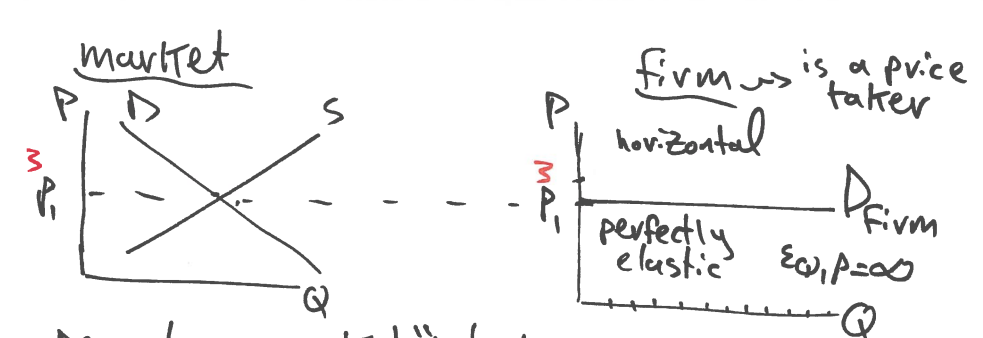
\includegraphics[width=\columnwidth]{../assets/demand-curve-pc.png}
  \caption{Demand Curve for Perfect Competition}
  \label{fig:demand_curve_pc}
\end{figure}

The demand curve for the market "industry" is negatively sloped. But the firm curve is horizontal.

The \textbf{Marginal Revenue} equals \textbf{Market Price} which is constant therefore \textbf{Total Revenue} increases at a constant rate.

\section{Profit maximizing for a firm}
There are two ways
\begin{enumerate}
  \item Total Revenue minus Total Cost approach
  \item Marginal Approach
\end{enumerate}

\subsection{Total Revenue and Total Cost}

\begin{Definition}
  {Profit}
  \begin{equation}
    \Pi = TR - TC 
  \end{equation}
  There are 3 cases 
  \begin{enumerate}
    \item $TR > TC$, $P > ATC$ or a profit
    \item $TR =  TC$, $P = ATC$ or a breakeven
    \item $TR < TC$, $P < ATC$ or a loss
  \end{enumerate}
  The objective of the firm is to maximize profit or $\Pi$ 

\end{Definition}
\begin{figure}[!h]
  \centering
  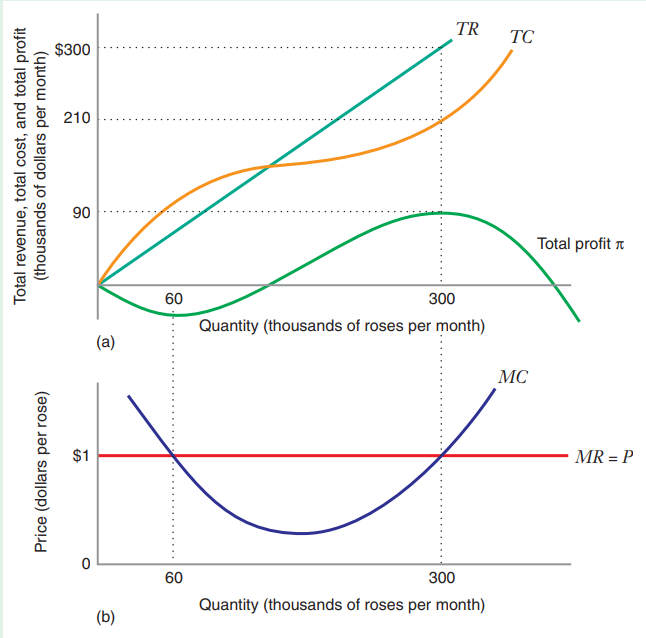
\includegraphics[width=\columnwidth]{../assets/PC-cost-curves.png}
  \caption{TR, TC, MR, MC curves}
  \label{fig:TR_TC_MR_MC_curves}
\end{figure}

\subsection{Marginal Approach}
Profit is maximized when:
\begin{enumerate}
  \item $MR = MC$, this is a necessary condition
  \item $MC$ is rising, this is a sufficient condition
\end{enumerate}
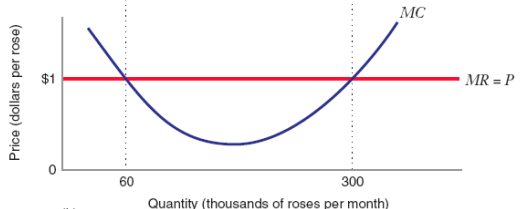
\includegraphics[width=\columnwidth]{assets/image-2021-12-11-12-02-43.png}
In the figure above the optimum quantity is at 300 and not 60 because the first quantity does not have a rising MC. Meaning if the producer keeps producing it will decrease the total cost \textbf{gained} for each unit produced increasing their overall profit.


\subsection{Cases based on Price}
There are five cases for profit based on the market price.
\begin{enumerate}
  \item Abnormal profit
  \item Breakeven "Normal Profit"
  \item Loss and continue
  \item Loss and indifferent
  \item Loss and shutdown
\end{enumerate}

\begin{figure}[!h]
  \centering
  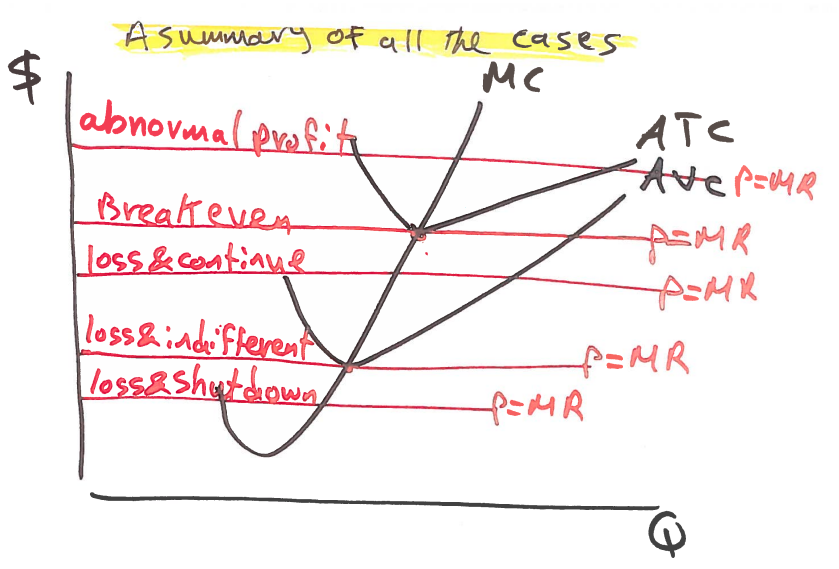
\includegraphics[width=\columnwidth]{../assets/summary_of_all_casses.png}
  \caption{The summary of all cases in Short Run}
  \label{fig:summary_of_all_cases_in_SR}
\end{figure}

\subsubsection{Abnormal profit}
Abnormal profit happens when $P > (ATC)$.
This is where the firm has a positive accounting and economic profit.

\subsubsection{Breakeven or Normal Profit}
Breakeven or normal profit occurs when $P = ATC$.
At this point there is zero economic profit however there is positive accounting profit.
In fact a zero economic profit is in fact a positive accounting profit or a "normal profit".

\subsubsection{Loss and Continue}
This happens when your $TC > TR > TVC$ or $(ATC) > P > (AVC)$, you can cover all of the variable cost and cover part of the total fixed cost. In this case it is better to continue and pay the uncovered part of $TFC$ out of pocket or from somewhere else like tapping into savings. 

\subsubsection{Loss and Indifferent}
This happens when your $TR = TVC$ or $(ATC) > P = (AVC)$, the loss between continuing and shutting down is the same so it doesn't matter if the firm continue or shutdown, that is why it is called indifferent.
The firm pays all of the $TFC$.
The $TR$ only pays the $TVC$ and nothing else.

\subsubsection{Loss and Shutdown}
This happens when your $TR < TVC$ or $(ATC) > (AVC) > P$, the loss from operating is higher than not operating at all so it would be better to shutdown and only pay the fixed cost $TFC$.
When $TR$ cannot cover $TVC$ the firm will shutdown because they cannot cover the variable cost of operation.

\section{Short Run Supply Curve of a Perfectly Competitive Firm}
Supply curve of a perfectly competitive firm is the rising part of the MC curve above the minimum $AVC$.
In \Cref{fig:SR_supply_curve} the bold line is the short run supply curve for the firm. The firm will not produce anything below the minimum of the \textbf{Average Variable Cost}.

\begin{figure}[!h]
  \centering
  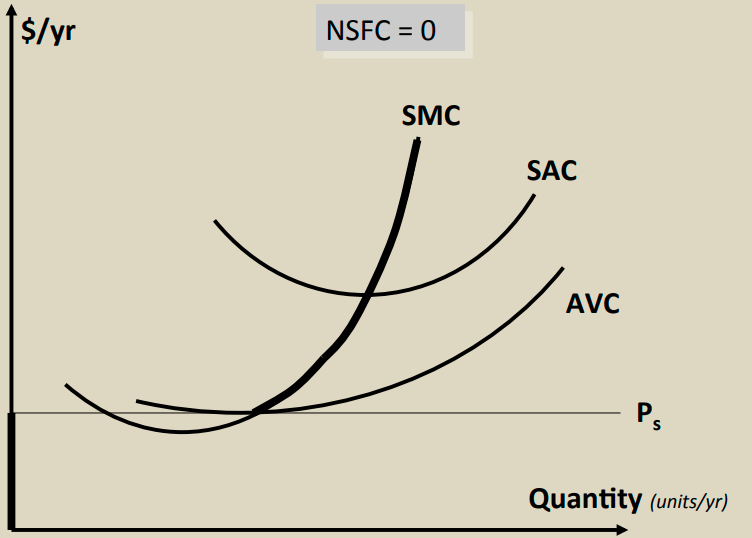
\includegraphics[width=\columnwidth]{assets/image-2021-12-11-12-07-15.png}
  \caption{Short Run Supply Curve}
  \label{fig:SR_supply_curve}
\end{figure}

\section{Long Run Equilibrium of a Competitive Firm}
In the long run the perfectly competitive firm will be making breakeven "normal profit" because of the free entry and exit into the market. 

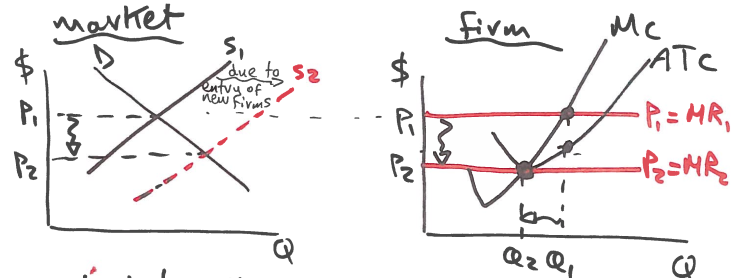
\includegraphics[width=\columnwidth]{assets/image-2021-12-11-12-10-51.png}

We started with having profits in the market. This will attracts new firms to enter the market, this will increase supply causing the supply curve to shift to the right so the price will decrease till we reach the breakeven price.

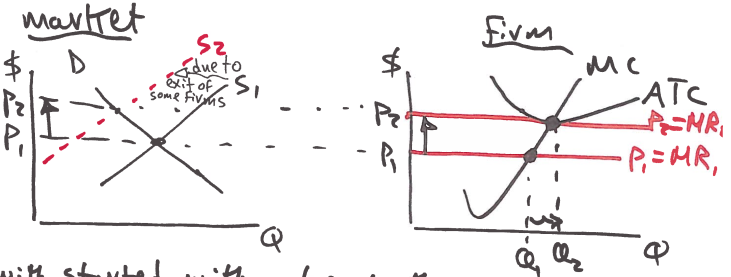
\includegraphics[width=\columnwidth]{assets/image-2021-12-11-12-11-09.png}

With started with a loss in the market. This loss will push some firms to exit or leave the market. This will decrease the supply and shift the supply curve to the left. This will increase the market price and the exit will continue as long as there is a loss and will stop once the loss disappear and we reach breakeven.
\newpage
\section{Efficiency}
We have 2 types of efficiency:
\begin{enumerate}
  \item Productive efficiency 
  \item Allocative efficiency
\end{enumerate}

\subsection{Productive efficiency}
To produce with the lowest ATC. 
\begin{Note}
  Notice that the perfectly competitive firm produces with the lowest LATC. So it achieves productive efficiency.
  Also at \(Q^*\) where \(P = LMC\) so it also achieves allocative efficiency
\end{Note}

\subsection{Allocative efficiency}
This happens when \(P = MC\)

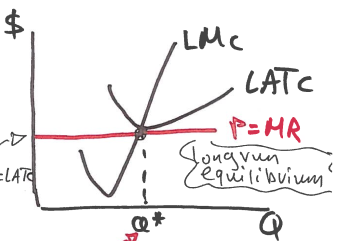
\includegraphics[width=\columnwidth]{assets/image-2021-12-11-12-15-21.png}

\newpage

\section{Competitive market}
In a perfectly competitive market, the competitive equilibrium quantity or \textbf{competitive quantity} will maximize total surplus or welfare.
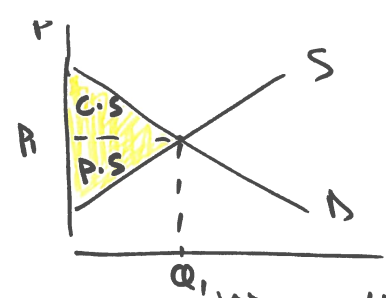
\includegraphics[width=\columnwidth]{assets/image-2021-12-11-12-18-36.png}

But any other quantity other than the equilibrium will give us less total surplus or a dead weight loss.
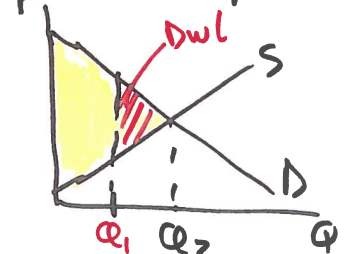
\includegraphics[width=\columnwidth]{assets/image-2021-12-11-12-18-54.png}




\end{document}
